\documentclass[11pt,a4paper]{article}

\usepackage[utf8]{inputenc}
\usepackage[T1]{fontenc}
\usepackage{amsmath,amssymb,bm}
\usepackage{graphicx}
\usepackage[margin=2.5cm]{geometry}
\usepackage[numbers,sort&compress]{natbib}
\usepackage{booktabs}
\usepackage{siunitx}
\usepackage{hyperref}
\usepackage{xcolor}

\graphicspath{{figures/}}

\newcommand{\todo}[1]{\textcolor{red}{[TODO: #1]}}
\newcommand{\soc}{\mathrm{SOC}}

\title{Joint state-of-charge and drifting current-sensor-bias estimation for
lithium-ion batteries: an augmented-state equivalent-circuit observer
evaluated against physics-based virtual cells}

\author{%
  Author One$^{a,\ast}$, Author Two$^{a}$\\[2pt]
  \small $^{a}$ Affiliation, Address\\
  \small $^{\ast}$ Corresponding author: \texttt{email@institution.edu}}
\date{}

\begin{document}
\maketitle

\begin{abstract}
\todo{Write after results are finalized.}
Accurate state-of-charge (SOC) estimation in battery management systems
relies on current and voltage measurements whose accuracy degrades over the
system lifetime. This work studies the joint estimation of SOC and a slowly
\emph{growing} current-measurement bias---originating from sensor ageing as
well as from un-modeled cabling and interconnection resistances---using an
equivalent-circuit-model (ECM) observer augmented with a bias state. The
observer is evaluated against physics-based virtual cells implemented in
PyBaMM with three published parameter sets (NMC, LCO and NMC/silicon--graphite
chemistries), under constant-current, CC--CV and dynamic-stress-test (DST)
operation, across temperature, C-rate, depth-of-discharge, drift-rate,
sensor-age and voltage-bias variations.
\todo{Add quantitative highlights and the experimental-validation summary.}
\end{abstract}

\section{Introduction}
\label{sec:intro}

The state of charge (SOC) of a lithium-ion battery is not directly
measurable and must be inferred from terminal quantities, most commonly by
combining coulomb counting with voltage-based correction in a model-based
observer---most commonly an equivalent-circuit model (ECM)
\citep{hu2012comparative} combined with an extended Kalman filter (EKF)
or one of its variants \citep{plett2004extended,plett2004extended2,%
plett2004extended3}. The fidelity of this inference is bounded by the
quality of the current and voltage measurements. While measurement
\emph{noise} is explicitly accommodated by the stochastic formulation of the
filter, measurement \emph{bias} is not: a systematic current offset is
integrated by the coulomb-counting dynamics and produces an unbounded drift
of the SOC estimate, while the voltage-based correction can only partially
counteract it, and may even be misled in flat regions of the open-circuit
voltage (OCV) curve. Comparative studies confirm that bias-type current
errors, unlike zero-mean noise, accumulate through the current integral and
can cause estimator divergence \citep{he2022comparative}, and error-source
surveys rank current-measurement offsets among the dominant contributors to
online SOC estimation error \citep{zheng2018investigating,truchot2014state}.
Lin \citep{lin2018theoretical} derived the SOC estimation bias and variance
as explicit functions of the sensor noises, the battery parameters and the
observer tuning, exposing a fundamental trade-off between suppressing the
bias-induced and the variance-induced error components---a trade-off that
an explicit bias state is designed to break.

Current-measurement bias in battery systems has several physical origins.
Hall-effect and shunt-based sensors exhibit offset errors that vary with
temperature and grow with ageing of the sensing element and its conditioning
electronics; calibration errors introduce quasi-static offsets that may
change abruptly after maintenance events. In addition, effects that are not
sensor faults at all can manifest as an equivalent measurement bias at the
observer level: un-modeled resistances of cabling, busbars, contact and
weld interfaces re-route or offset the effective current seen by the model,
and their slow growth with interconnect ageing produces a bias-like,
time-varying disturbance. From the observer's perspective these
contributions lump into a single, slowly drifting disturbance term, which
motivates estimating it online rather than assuming it constant or zero.

The idea of augmenting a battery state estimator with sensor-bias states is
established. Zhao et al.\ \citep{zhao2017observability} derived necessary
and sufficient observability conditions for a nonlinear ECM using a
differential-geometric approach, and demonstrated---including experimental
validation on an NMC pouch cell---that current- and voltage-sensor biases
can be estimated by a nonlinear Kalman filter acting on an augmented model;
importantly, they also showed that the simultaneous estimation of both
current- and voltage-sensor biases renders the SOC ambiguous, since the
filter cannot attribute an output error to one sensor or the other. Yoo et
al.\ \citep{yoo2023uam} developed an EKF-based current-sensor bias
estimator for a hybrid urban-air-mobility application and validated it with
Hall-sensor measurements, maintaining SOC errors within \SI{2}{\percent}
under realistic flight profiles. Dual-filter formulations that decouple the
bias estimate from the electrochemical states have recently been proposed
for chemistries with flat OCV characteristics \citep{guo2025rbc}. Beyond
estimation, the fault-diagnosis literature treats sensor bias as one of
several fault classes (bias, gain, drift, intermittent) to be detected and
reconstructed by dedicated observers \citep{lan2023sensor}.

Three gaps remain. First, the bias is almost universally modeled and
injected as a \emph{constant} (or step) offset, whereas the degradation
mechanisms above produce a bias that \emph{grows in time}, on time scales
comparable to or slower than a single operating cycle; the ability of an
augmented observer to \emph{track} such drift, and the excitation it
requires, is not systematically characterized. Second, validation is
typically performed on a single cell and chemistry; since the bias enters
the measurement equation through the ohmic resistance and the OCV slope,
its identifiability is strongly chemistry- and operating-point-dependent,
which calls for a controlled multi-chemistry assessment. Third, synthetic
studies usually corrupt data generated by the \emph{same} model class used
by the observer, hiding the interaction between model mismatch and bias
estimation; a physics-based plant of a different model class provides a
more honest testbed.

This paper addresses these gaps with the following contributions:
\begin{enumerate}
  \item a simulation framework in which the plant is a physics-based
        single-particle model with electrolyte (SPMe) implemented in PyBaMM
        \citep{sulzer2021pybamm}, instantiated with three published
        parameter sets---Mohtat2020 \citep{mohtat2020}, Ai2020
        \citep{ai2020} and OKane2022 \citep{okane2022} (based on the LG M50
        parameterization of Chen et al.\ \citep{chen2020})---while the
        observer uses a deliberately mismatched second-order ECM;
  \item a sensor-degradation model comprising an initial offset (``sensor
        age''), a slow drift in time, step faults and random-walk
        components on the current channel, and a constant or drifting bias
        on the voltage channel, with magnitudes anchored to published
        datasheet figures for automotive current sensing
        \citep{melexis2023shunt}; observers augmented with the current
        bias, the voltage bias, or both are compared, the last probing the
        ambiguity of \citep{zhao2017observability} quantitatively;
  \item a joint battery-aging / sensor-aging study in which aged virtual
        cells (loss of active material and ohmic resistance growth, down to
        \SI{80}{\percent} SOH) are observed with the fresh-cell
        calibration, quantifying both the growing benefit of the bias state
        and the confounding between sensor diagnosis and aging;
  \item a bias-augmented EKF on the ECM, compared one-to-one against its
        non-augmented counterpart over a full-factorial-inspired campaign
        spanning chemistry, load profile (constant current, CC--CV cycle,
        and a dynamic stress test scaled from the USABC procedure
        \citep{usabc1996}), temperature, peak C-rate, depth of discharge,
        drift rate, sensor age and voltage bias;
  \item a joint battery-ageing $\times$ sensor-ageing campaign in which
        the plant is aged (loss of active material and resistance growth)
        while the observer retains its beginning-of-life calibration,
        demonstrating that the value of the bias state \emph{grows} with
        battery age: the estimated bias absorbs the lumped disturbance
        created by capacity fade and resistance growth in addition to the
        physical sensor offset, keeping the SOC error bounded where the
        baseline observer degrades;
  \item \todo{experimental validation on a laboratory cell tester with
        software-injected, ground-truth-known drifting bias and a physical
        series resistance in the cabling.}
\end{enumerate}

The remainder of the paper is organized as follows.
Section~\ref{sec:method} describes the virtual plant, the observer models,
the sensor-degradation models and the design of the simulation campaign.
Section~\ref{sec:results} reports the results. Section~\ref{sec:conclusion}
concludes.

\section{Methodology}
\label{sec:method}

\subsection{Physics-based virtual plant}
\label{sec:plant}

The plant is the single-particle model with electrolyte dynamics (SPMe)
\citep{marquis2019asymptotic}---a reduced-order descendant of the
Doyle--Fuller--Newman model \citep{doyle1993modeling}---as
implemented in PyBaMM v26 \citep{sulzer2021pybamm}, solved isothermally at a
prescribed ambient temperature $T$. Three published parameter sets are
used, providing chemically distinct virtual cells: Mohtat2020 (\SI{5}{Ah}
NMC/graphite pouch cell \citep{mohtat2020}), Ai2020 (\SI{2.28}{Ah}
LCO/graphite pouch cell \citep{ai2020}) and OKane2022 (\SI{5}{Ah} NMC811 /
silicon--graphite cylindrical cell \citep{okane2022,chen2020}). Using a
physics-based plant of a different model class than the observer introduces
a realistic, structured model mismatch: the residual voltage error of the
calibrated observer model against the plant is \SIrange{13}{30}{mV} RMS
depending on chemistry and temperature (Section~\ref{sec:calibration}),
comparable to what is observed when fitting ECMs to laboratory data.

\subsection{Observer model and calibration}
\label{sec:calibration}

The observer uses a second-order ECM. With the PyBaMM sign convention
($i>0$ in discharge), the continuous-time model is
\begin{align}
  \dot{\soc} &= -\frac{i}{3600\,Q}, &
  \dot{v}_j &= -\frac{v_j}{\tau_j} + \frac{R_j}{\tau_j}\, i, \quad j=1,2,
  \label{eq:ecm-states}\\
  v &= U(\soc) - R_0\, i - v_1 - v_2,
  \label{eq:ecm-output}
\end{align}
where $Q$ is the usable capacity, $U(\cdot)$ the pseudo-OCV curve, $R_0$
the ohmic resistance and $(R_j,\tau_j)$ the RC polarization branches.

The pseudo-OCV curve is obtained from the plant by a C/25
discharge--charge pair between the voltage limits, taking the mean of the
two branches on a common SOC axis. Averaging the branches removes both the
small residual overpotential and the OCV hysteresis, which is significant
for the silicon-containing negative electrode of the OKane2022 cell. The
usable capacity $Q$ is defined as the charge throughput of the C/25
discharge branch, and SOC is referenced to this window throughout.

The ECM parameters $\theta = (R_0, R_1, \tau_1, R_2, \tau_2)$ are
calibrated by nonlinear least squares against \emph{bias-free
commissioning data}: a \SI{1}{C} constant-current discharge of the plant at
the operating temperature. The simulated ECM terminal voltage, driven by
the true current and evaluated at the true SOC, is fitted to the plant
voltage with a trust-region-reflective solver under box constraints, and
samples below \SI{5}{\percent} SOC are excluded to prevent the steep OCV
tail from dominating the cost. This mimics the realistic workflow in which
the model is calibrated when the pack is new and the instrumentation
trusted, and subsequently deployed while the sensors degrade. The
calibration is repeated for every (chemistry, temperature) pair used in the
campaign.

\subsection{Sensor degradation model}
\label{sec:sensors}

The observer receives corrupted measurements
\begin{align}
  i_m(t) &= i(t) + b(t) + w_i(t), &
  v_m(t) &= v(t) + b_v(t) + w_v(t),
\end{align}
with zero-mean white noises $w_i \sim \mathcal{N}(0,\sigma_i^2)$,
$w_v \sim \mathcal{N}(0,\sigma_v^2)$
($\sigma_i = \SI{20}{mA}$, $\sigma_v = \SI{2}{mV}$). The current-sensor
bias is modeled as
\begin{equation}
  b(t) = b_0 + \dot{b}\,t + \Delta b\,\mathbb{1}(t \ge t_s) + \beta(t),
  \label{eq:bias-model}
\end{equation}
where $b_0$ is the offset accumulated before the test (``sensor age''),
$\dot{b}$ a constant drift rate representing slow degradation of the
sensor and of the interconnect resistances, $\Delta b$ an optional step
(calibration-type fault) at time $t_s$, and $\beta(t)$ an optional Wiener
process. The magnitudes are chosen to be representative of automotive-grade
instrumentation: open-loop Hall-effect pack-current sensors exhibit offset
errors of the order of \SIrange{0.5}{1}{\percent} of full scale, with a
residual offset that drifts with temperature, package stress and ageing
even after factory compensation \citep{allegro_hall}; for a
\SIrange{15}{25}{A} full-scale sensor this corresponds to
$b_0 \approx$ \SIrange{0.1}{0.25}{A}, while the within-test drift---
dominated by the thermal excursion of the sensor during operation---is of
the order of tens of \si{mA} per hour. The baseline scenario therefore
uses $b_0 = \SI{0.1}{A}$ and $\dot b = \SI{0.02}{A/h}$, with sweeps from
\SI{0.005}{A/h} to \SI{0.05}{A/h} and a dedicated \SI{0.1}{A}
step-fault case. The voltage-sensor bias $b_v(t)$ is constant or slowly drifting.

The magnitudes are anchored to published figures for automotive sensing:
Hall-effect and shunt current sensors exhibit lifetime offset and
sensitivity drifts of the order of \SIrange{0.1}{1}{\percent} of full
scale \citep{melexis2023shunt}, i.e.\ tens to a few hundred
\si{\milli\ampere} for a cell-level sensor, accumulating over months of
operation; battery-monitoring analog front ends specify total voltage
measurement errors of \SIrange{1}{2}{\milli\volt}. Within a single test
the physical drift is therefore quasi-static and is represented by the
initial offset $b_0$, which grows across life stages; scenarios with
in-test drift rates $\dot b \ge \SI{0.05}{A/h}$ are labeled
\emph{accelerated} and serve as stress tests of the drift-tracking
bandwidth. Larger lumped offsets remain plausible when un-modeled cabling
and interconnect resistances contribute, which is precisely the
lumped-disturbance interpretation adopted here.

\subsection{Battery aging emulation}
\label{sec:aging}

To study the interaction between sensor degradation and battery
degradation, aged virtual cells are generated from the fresh parameter
sets by two mechanisms. Loss of active material (LAM) is emulated by
scaling the active-material volume fractions of both electrodes by a
factor equal to the target state of health (SOH), producing an
approximately proportional capacity fade. Ohmic resistance growth---the
lumped effect of SEI growth and of contact/interconnect degradation---is
applied as an exact series resistance
$\Delta R = 2\,R_0^{\mathrm{fresh}}\,(1 - \mathrm{SOH})$
on the terminal voltage. SOH levels of \SIlist{100;95;90;85;80}{\percent}
are considered. Crucially, the observer retains the \emph{fresh}
calibration ($Q$, ECM parameters and pseudo-OCV) at all SOH levels,
reproducing the realistic situation of a BMS whose model has not been
re-identified as the pack ages. The true SOC of the aged cell is
referenced to the aged usable capacity. This design probes the
lumped-disturbance interpretation of the bias state: capacity fade injects
a coulombic error and resistance growth injects a voltage error, both of
which the augmented filter can partially absorb into $\hat b$---improving
SOC accuracy at the cost of biasing the sensor-fault diagnosis, a
confounding that is quantified in Section~\ref{sec:results}.

\subsection{Bias-augmented extended Kalman filter}
\label{sec:ekf}

Discretizing \eqref{eq:ecm-states} exactly over a step $\Delta t_k$ and
augmenting the state with the bias, modeled as a random walk, gives
$x_k = [\soc_k,\, v_{1,k},\, v_{2,k},\, b_k]^\top$ with
\begin{align}
  \soc_{k+1} &= \soc_k - \frac{(i_{m,k} - b_k)\,\Delta t_k}{3600\,Q}, \\
  v_{j,k+1} &= a_{j,k}\, v_{j,k} + R_j\,(1 - a_{j,k})\,(i_{m,k} - b_k),
  \qquad a_{j,k} = e^{-\Delta t_k / \tau_j}, \\
  b_{k+1} &= b_k + \eta_k, \qquad \eta_k \sim \mathcal{N}(0, q_b),
\end{align}
and measurement model
\begin{equation}
  v_{m,k} = U(\soc_k) - R_0\,(i_{m,k} - b_k) - v_{1,k} - v_{2,k} + w_{v,k}.
  \label{eq:meas}
\end{equation}
The measurement Jacobian is
$H_k = [\partial U/\partial\soc,\; -1,\; -1,\; R_0]$: the bias is
instantaneously observable through the ohmic term $R_0 b_k$ and, on longer
horizons, through the coulombic channel
$\partial \soc_{k+1}/\partial b_k = \Delta t_k / (3600\,Q)$ weighted by the
local OCV slope. Both channels degrade in flat OCV regions and for
low-impedance cells, which is the mechanistic origin of the
chemistry dependence investigated in the campaign. Analogously, a voltage-sensor-bias state $b_{v,k}$ can be
appended (measurement Jacobian entry $\partial v / \partial b_v = 1$),
either instead of or in addition to $b_k$; the filter with both bias states
is included deliberately, as the simultaneous case is known to make the SOC
unobservable in principle \citep{zhao2017observability}, and the campaign
quantifies the practical consequences. The process noise of
the bias state, $q_b$, sets the drift-tracking bandwidth of the filter, and
the measurement variance is inflated above the true sensor noise
($r_v = \SI{2.5e-5}{V^2}$, i.e.\ an effective \SI{5}{mV} standard
deviation) to absorb the residual ECM model error and prevent it from being
misattributed to the bias state. The observer can additionally (or alternatively) be augmented with a
voltage-sensor bias state $b_{v,k}$, also modeled as a random walk, which
enters the measurement model \eqref{eq:meas} additively with Jacobian
entry $+1$. Estimating both $b$ and $b_v$ simultaneously is known to make
the SOC weakly identifiable \citep{zhao2017observability}; the campaign
quantifies this cost empirically by comparing the $\{b\}$-,
$\{b_v\}$- and $\{b, b_v\}$-augmented variants. The baseline observer
is the identical EKF without any bias state; all filters are initialized
with a deliberate SOC error to also assess convergence.

\subsection{Battery ageing emulation}
\label{sec:aging}

Battery ageing is emulated in the plant by two controlled mechanisms:
capacity fade, implemented as a proportional loss of active material in
both electrodes (the active-material volume fractions are scaled by the
target state of health, SOH), and resistance growth, implemented as an
additional series resistance $\Delta R$ applied to the terminal voltage,
representing aged interfaces, welds and cabling. Five life stages are
defined, jointly degrading the battery and the sensors:
SOH $\in \{100, 95, 90, 85, 80\}\,\%$, $\Delta R \in
\{0, 15, 30, 45, 60\}\,\%$ of the beginning-of-life (BOL) $R_0$,
current-sensor offset $b_0 \in \{10, 40, 80, 110, 150\}$\,mA and
voltage-sensor offset $b_v \in \{0.5, 1, 2, 3, 5\}$\,mV. The true
usable capacity of each aged cell is measured by a C/25 discharge of the
aged plant, while the observer retains its BOL calibration ($Q$, ECM
parameters and OCV)---the realistic situation of a BMS without online
capacity adaptation. Note that with the BOL capacity in the
coulomb-counting equation, capacity fade produces a state-equation error
proportional to the current, whose running mean is absorbed by the bias
state; the bias estimate therefore acquires the meaning of a
\emph{lumped ageing-and-sensor disturbance} rather than a pure sensor
offset, which is quantified in the results.

\subsection{Load profiles}
\label{sec:profiles}

Three load profiles are used. (i)~A \SI{1}{C} constant-current (CC)
discharge from \SI{100}{\percent} SOC to the voltage cut-off. (ii)~A full
CC--CV cycle: \SI{1}{C} discharge, \SI{10}{min} rest, \SI{0.5}{C} charge
with a \SI{4.2}{V} constant-voltage hold to a C/50 cut, and a final rest.
(iii)~A dynamic stress test (DST) in the spirit of the USABC procedure
\citep{usabc1996}: the \SI{92}{s} base sequence of discharge, rest and
regenerative-charge steps is first normalized so that its peak discharge
magnitude equals one, then scaled such that the peak reaches a prescribed
C-rate, and repeated until a target depth of discharge (DoD) or the voltage
cut-off is reached. The DST is applied after a CC--CV charge
(\SI{0.5}{C}, \SI{4.2}{V}, C/50 cut) so that each dynamic test starts from
a well-defined full state. Figure~\ref{fig:dst} shows the scaled profile.

\begin{figure}[t]
  \centering
  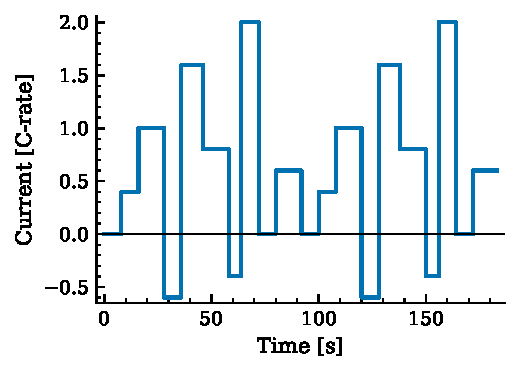
\includegraphics{fig_dst_profile.pdf}
  \caption{Two periods of the DST current profile, normalized to its peak
  discharge magnitude and scaled to a \SI{2}{C} peak (positive = discharge).}
  \label{fig:dst}
\end{figure}

\begin{figure}[t]
  \centering
  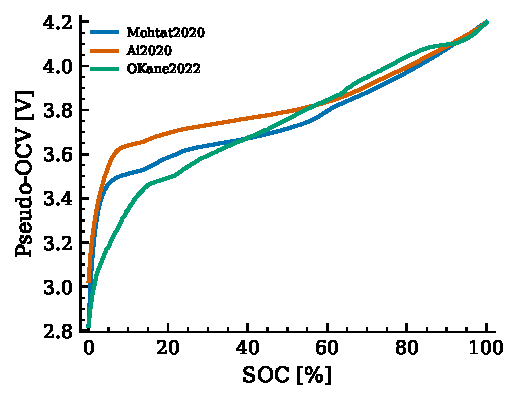
\includegraphics{fig_ocv.pdf}
  \caption{Pseudo-OCV curves of the three virtual cells (mean of C/25
  charge and discharge branches, \SI{25}{\celsius}).}
  \label{fig:ocv}
\end{figure}

\subsection{Simulation campaign and metrics}
\label{sec:campaign}

The campaign combines a baseline scenario (DST with \SI{2}{C} peak,
\SI{80}{\percent} DoD, \SI{25}{\celsius}, drift
$\dot b = \SI{0.15}{A/h}$ plus a \SI{0.1}{A} mid-test step, $b_0 = 0$,
$b_v = 0$) with one-factor-at-a-time sweeps: chemistry and profile
(3~parameter sets $\times$ \{CC, CC--CV, DST\}), temperature
(\SIlist{10;25;40}{\celsius}), DST peak C-rate (1--3C), DoD
(\SIrange{50}{95}{\percent}), drift rate (\SIrange{0.05}{0.60}{A/h}),
sensor age ($b_0 \in \{0, 0.2, 0.5\}$\,A) and voltage bias
($b_v = \SI{5}{mV}$, alone and combined with current drift), a
datasheet-consistent \emph{realistic} scenario ($b_0 = \SI{50}{mA}$,
$\dot b = \SI{5}{mA/h}$, $b_v = \SI{1}{mV}$), and the five-stage joint
ageing campaign of Section~\ref{sec:aging}, for 28 cases in total. Every case is run with both the baseline and the augmented EKF
under identical tuning, noise realizations and (wrong) initialization.
Performance is quantified by the SOC root-mean-square error (RMSE) and
maximum absolute error after a \SI{120}{s} transient, and by the RMSE of
the bias estimate against the injected ground truth. All raw time series
are stored, and all figures and tables in Section~\ref{sec:results} are
generated programmatically from them.

\section{Results}
\label{sec:results}

\todo{Results section intentionally left empty. The figures and the table
below are auto-generated by \texttt{postprocess.py} from the campaign in
\texttt{run\_experiments.py}; write the discussion around them.}

\subsection{Chemistry and load-profile dependence}
\begin{figure}[t]
  \centering
  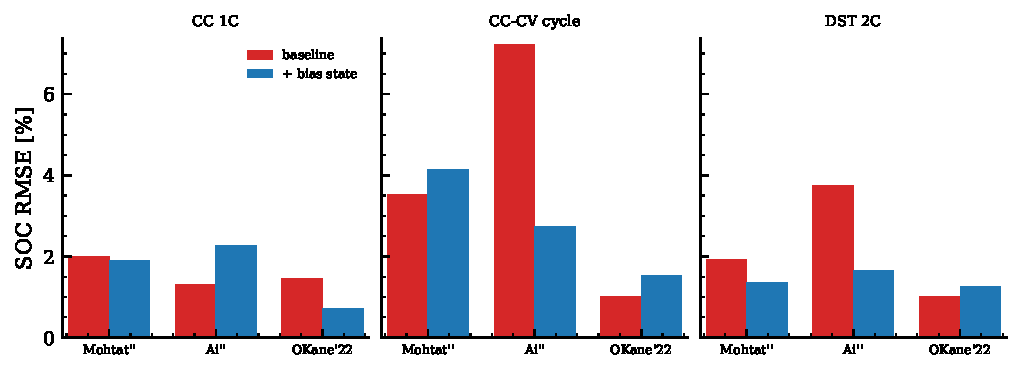
\includegraphics{fig_chemistry.pdf}
  \caption{SOC RMSE of the baseline and bias-augmented EKF for the three
  chemistries under CC, CC--CV and DST operation (baseline bias scenario).}
  \label{fig:chemistry}
\end{figure}

\begin{figure}[t]
  \centering
  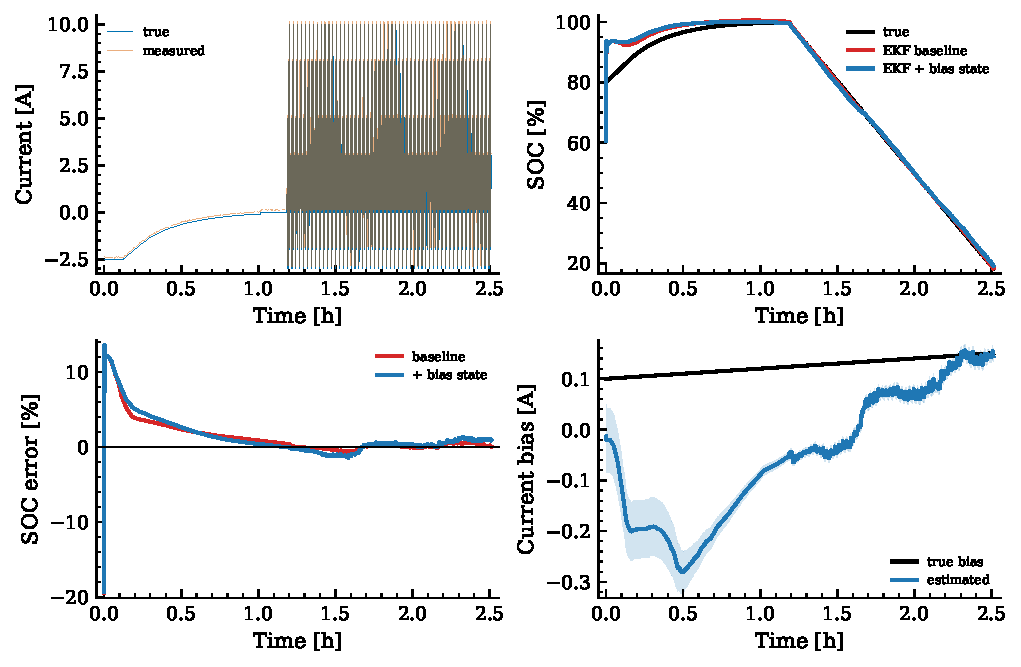
\includegraphics{fig_timeseries_okane_dst.pdf}
  \caption{Representative DST case (OKane2022, \SI{2}{C} peak,
  \SI{25}{\celsius}): measured vs.\ true current, SOC estimates, SOC
  errors, and bias tracking with $\pm 2\sigma$ credible band.}
  \label{fig:timeseries}
\end{figure}

\subsection{Operating-condition sweeps}
\begin{figure}[t]
  \centering
  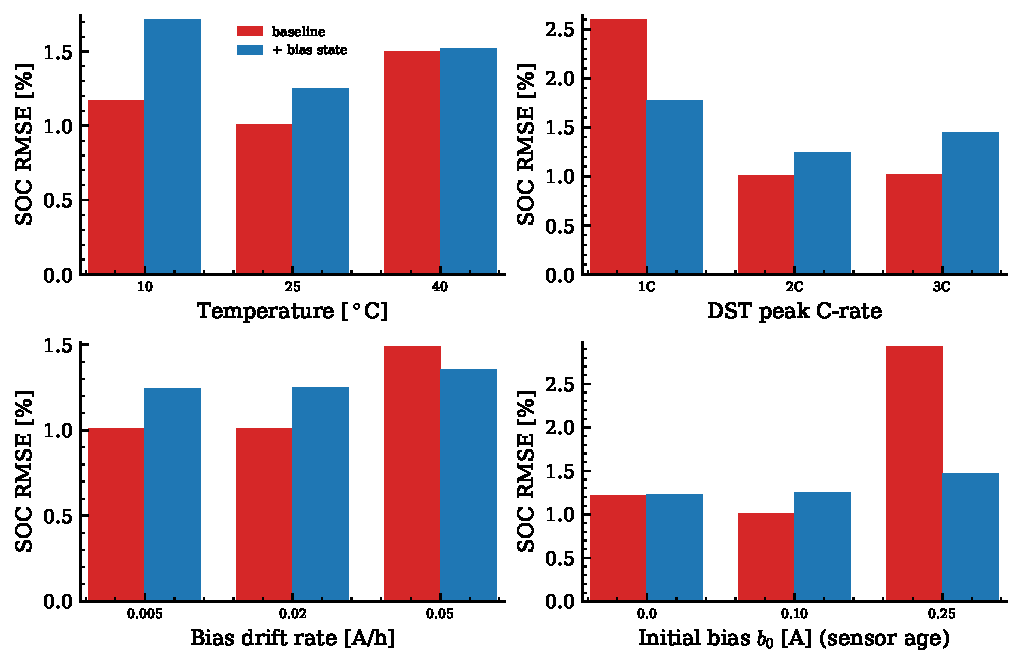
\includegraphics{fig_sweeps.pdf}
  \caption{One-factor-at-a-time sweeps (OKane2022, DST): temperature, DST
  peak C-rate, bias drift rate and sensor age.}
  \label{fig:sweeps}
\end{figure}

\subsection{Drift tracking}
\begin{figure}[t]
  \centering
  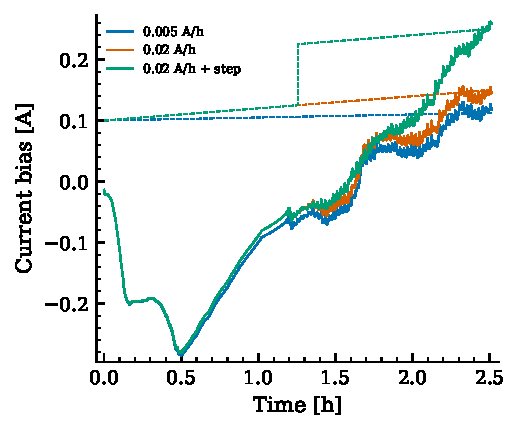
\includegraphics{fig_bias_tracking.pdf}
  \caption{Estimated (solid) vs.\ true (dashed) current-sensor bias for
  three drift rates.}
  \label{fig:tracking}
\end{figure}

\subsection{Interaction with battery ageing}
\begin{figure}[t]
  \centering
  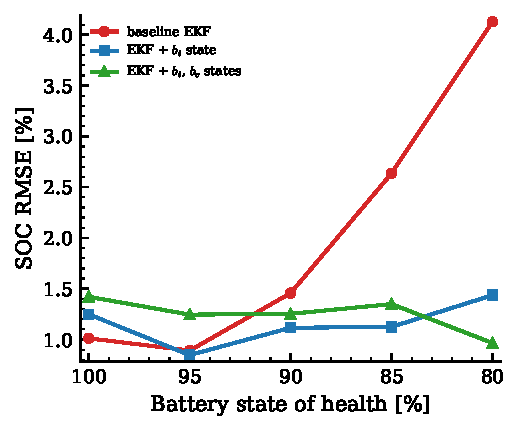
\includegraphics{fig_aging.pdf}
  \caption{Joint battery-ageing $\times$ sensor-ageing campaign
  (OKane2022, DST \SI{2}{C} peak): SOC RMSE of the baseline EKF and of
  the variants augmented with the current-sensor bias state and with both
  bias states, as a function of battery state of health. The observer
  retains its beginning-of-life calibration at all stages.}
  \label{fig:aging}
\end{figure}

\begin{figure}[t]
  \centering
  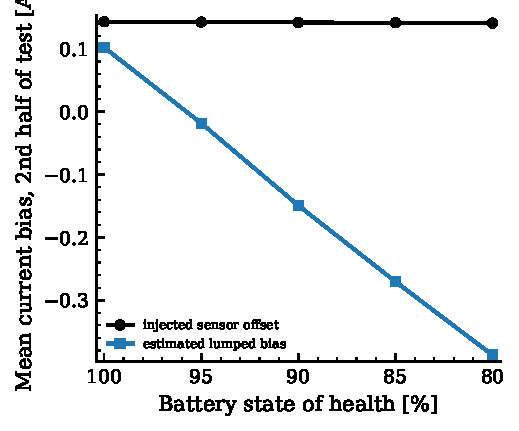
\includegraphics{fig_aging_bias.pdf}
  \caption{Mean estimated lumped bias over the second half of each test
  vs.\ the injected physical sensor offset, across life stages: the bias
  state increasingly absorbs ageing-induced disturbances (capacity fade,
  resistance growth) on top of the sensor offset.}
  \label{fig:aging-bias}
\end{figure}

\subsection{Interaction with battery aging}
\begin{figure}[t]
  \centering
  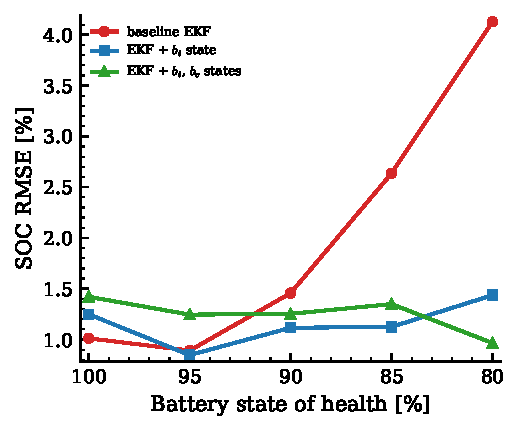
\includegraphics{fig_aging.pdf}
  \caption{SOC RMSE vs.\ battery SOH for the baseline, current-bias
  augmented, and dual-bias EKF; observer calibration is kept at the fresh
  state throughout.}
  \label{fig:aging}
\end{figure}

\begin{figure}[t]
  \centering
  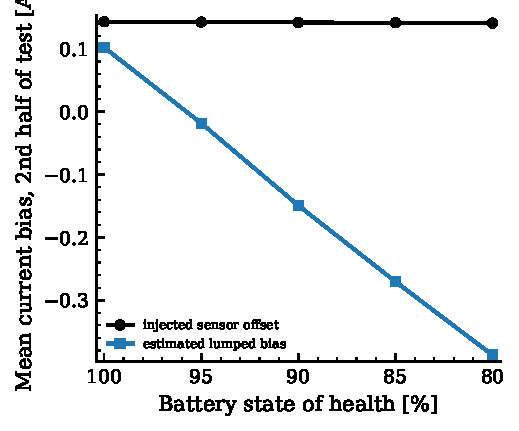
\includegraphics{fig_aging_bias.pdf}
  \caption{Injected sensor offset vs.\ estimated lumped bias across SOH
  levels: the bias state absorbs aging-induced disturbances beyond the true
  sensor offset (diagnosis/accuracy confounding).}
  \label{fig:aging_bias}
\end{figure}

\subsection{Current/voltage bias ambiguity}
\begin{figure}[t]
  \centering
  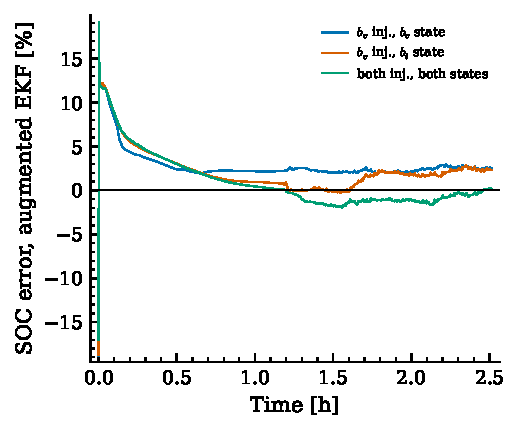
\includegraphics{fig_vbias.pdf}
  \caption{SOC error of the augmented EKF when a \SI{5}{mV} voltage-sensor
  bias is present, alone and combined with current drift.}
  \label{fig:vbias}
\end{figure}

% Auto-generated by postprocess.py -- do not edit by hand
\begin{table*}[t]
\centering
\caption{Summary of all simulation cases. RMSE values computed after a 120\,s transient. Baseline: EKF without bias state; augmented: EKF with current-bias state.}
\label{tab:summary}
\small
\begin{tabular}{llrrrrrrr}
\hline
Case & Profile & $T$ [$^\circ$C] & drift [A/h] & $b_0$ [A] & $b_v$ [mV] & RMSE$_\mathrm{base}$ [\%] & RMSE$_\mathrm{aug}$ [\%] & bias RMSE [mA] \\
\hline
Mohtat2020\_cc & cc & 25 & 0.02 & 0.1 & 0 & 2.01 & 1.90 & 93 \\
Mohtat2020\_cccv & cccv & 25 & 0.02 & 0.1 & 0 & 3.54 & 4.15 & 214 \\
Mohtat2020\_dst & dst & 25 & 0.02 & 0.1 & 0 & 1.92 & 1.36 & 104 \\
Ai2020\_cc & cc & 25 & 0.02 & 0.1 & 0 & 1.32 & 2.28 & 55 \\
Ai2020\_cccv & cccv & 25 & 0.02 & 0.1 & 0 & 7.22 & 2.74 & 63 \\
Ai2020\_dst & dst & 25 & 0.02 & 0.1 & 0 & 3.74 & 1.64 & 55 \\
OKane2022\_cc & cc & 25 & 0.02 & 0.1 & 0 & 1.45 & 0.71 & 131 \\
OKane2022\_cccv & cccv & 25 & 0.02 & 0.1 & 0 & 1.01 & 1.52 & 87 \\
OKane2022\_dst & dst & 25 & 0.02 & 0.1 & 0 & 1.01 & 1.25 & 130 \\
OKane2022\_dst\_T10 & dst & 10 & 0.02 & 0.1 & 0 & 1.17 & 1.71 & 78 \\
OKane2022\_dst\_T40 & dst & 40 & 0.02 & 0.1 & 0 & 1.50 & 1.52 & 154 \\
OKane2022\_dst\_peak1C & dst & 25 & 0.02 & 0.1 & 0 & 2.60 & 1.77 & 114 \\
OKane2022\_dst\_peak3C & dst & 25 & 0.02 & 0.1 & 0 & 1.02 & 1.45 & 150 \\
OKane2022\_dst\_dod50 & dst & 25 & 0.02 & 0.1 & 0 & 0.95 & 0.98 & 132 \\
OKane2022\_dst\_dod95 & dst & 25 & 0.02 & 0.1 & 0 & 1.01 & 0.87 & 102 \\
OKane2022\_dst\_drift0p005 & dst & 25 & 0.01 & 0.1 & 0 & 1.01 & 1.25 & 125 \\
OKane2022\_dst\_drift0p05 & dst & 25 & 0.05 & 0.1 & 0 & 1.49 & 1.35 & 150 \\
OKane2022\_dst\_stepfault & dst & 25 & 0.02 & 0.1 & 0 & 1.78 & 1.45 & 185 \\
OKane2022\_dst\_age0p0 & dst & 25 & 0.02 & 0.0 & 0 & 1.22 & 1.23 & 126 \\
OKane2022\_dst\_age0p25 & dst & 25 & 0.02 & 0.2 & 0 & 2.92 & 1.47 & 165 \\
OKane2022\_dst\_vbias5mV\_obsV & dst & 25 & 0.00 & 0.0 & 5 & 2.23 & 2.49 & 0 \\
OKane2022\_dst\_vbias5mV\_obsI & dst & 25 & 0.00 & 0.0 & 5 & 2.23 & 1.92 & 111 \\
OKane2022\_dst\_bothbias\_obsIV & dst & 25 & 0.02 & 0.1 & 5 & 0.81 & 1.56 & 149 \\
OKane2022\_dst\_soh100 & dst & 25 & 0.02 & 0.1 & 0 & 1.01 & 1.25 & 130 \\
OKane2022\_dst\_soh95 & dst & 25 & 0.02 & 0.1 & 0 & 0.89 & 0.85 & 174 \\
OKane2022\_dst\_soh90 & dst & 25 & 0.02 & 0.1 & 0 & 1.46 & 1.12 & 277 \\
OKane2022\_dst\_soh85 & dst & 25 & 0.02 & 0.1 & 0 & 2.64 & 1.12 & 367 \\
OKane2022\_dst\_soh80 & dst & 25 & 0.02 & 0.1 & 0 & 4.13 & 1.44 & 465 \\
\hline
\end{tabular}
\end{table*}


\subsection{Experimental validation}
\todo{Add experimental validation on the laboratory tester:
software-injected drifting bias with ground truth from a reference shunt,
and a physical series resistance inserted in the cabling.}

\section{Conclusions}
\label{sec:conclusion}
\todo{Write after results.}

\section*{Acknowledgments}
\todo{Funding and acknowledgments.}

\bibliographystyle{unsrtnat}
\bibliography{references}

\end{document}
